\documentclass[10pt,conference]{IEEEtran}

\usepackage{hyperref}
\usepackage{graphicx}
\usepackage{xcolor}
\usepackage{blindtext, amsmath, comment, subfig, epsfig }
\usepackage{grffile}
\usepackage{caption}
%\usepackage{subcaption}
\usepackage{algorithmic}
\usepackage[utf8]{inputenc}


\title{CS523 Project 1 Report}
\author{Wicky Simon, Nunes Silva Daniel Filipe}
\date{February 2020}

\begin{document}

\maketitle

\begin{abstract}
This project consists in the implementation a $N$-party multiparty
computations system. Unlike a traditional approach, this aims to compute
the result of a given circuit using users secret inputs without requiring
them to reveal them explicitely. To achieve it, our Go program must be runned
by each of the users who provide their secret values and the ciruit they
want to compute together. Then, they share their additive secret sharings
across the network they are linked with, parse the circuit, generate Beaver
triplets when necessary and evaluate the result before retrieving it.
We analyze the scenarios and the consequenting tradeoffs in which the users
have access to a trusted third-party and the one in which they have not. We
make use of the Lattigo library for the cryptographic operations and the
algebraic structure implementations it provides.

%Please report your design, implementation details, findings of the first project in this report. \\
You can add references if necessary \cite{article}. \\
%THE REPORT SHOULD NOT EXCEED 3 PAGES.
\end{abstract}
\section{Introduction}
The aim of this project is to design, implement and assess two MPC engines using
the Go programming language. First, two weeks are dedicated to the understanding
of the general architecture, how to use it and how to tweak it to perform
computations in a privacy preserving fashion. We implement the additive secret
sharings split of the secrets, the circuit parsing, the corresponding gates, the
Beaver triplets generation, update the network operations and describe our own
complex circuit assuming the presence of a trusted third party during the two
following weeks. Two more weeks to adapt our system so that it is able to
generate Beaver triplets with no trusted third party but using BFV homomorphic
encryption handled by Lattigo. Finally, we dedicate one week to revise our
implementations, compare and evaluate them.

%Give a brief introduction about the aim of the project, and your road-map about the design/implementation.
\section{Part I}

\subsection{Threat model}
The asset to protect for a party is the input. During the protocl, anyone monitoring the communication should not be able to recover the input of a given party. In particular, a party taking part in the computation can not infer more information about another party's input that what he could have infered if all data had been sent to a trusted third-party making the computation for them and sending the result.

All parties follow the "honest but curious" threat model. They do not deviate from the protocol and compute the correct circuit, but try to infer informations about other's input.

Furthermore, a third-party is trusted to generate the beaver triplets, necessary for the computation of multiplications.

%Give the corresponding threat model for the first part of the project that you implemented. 
\subsection{Implementation details}
\begin{itemize}
    \item \textit{main.go} : This file is the entry point of the programm. It handles the creation of a party, the set up of the network, the circuit and launch the computation. The structure has been slightly adapted from the handout, to fit the changes made. Note that since each party runs independently, this file is unused in the first part, since the beaver triplets are generated in a single location.
    \item \textit{helper.go} : This file contains two helper methods :
        \begin{itemize}
            \item Pmod(x,mod) : computes x modulo mod. This method is necessary because the \% operator can return negative results.
            \item secret\_share(secret,n) : Split a secret into $n$ parts using additive sharing.
        \end{itemize}
    \item \textit{gates.go} : Implements the different gates needed for the circuits.
    \item \textit{circuits.go} : Contains two methods :
        \begin{itemize}
            \item SetUpMPC(circuit, trusted) : Create the necessary structure for the protocol to run, and generate the beaver triplets depending on the chosen setting for \textit{trusted}. This setting is used for modularity between Part 1 and Part 2. During this set up, the circuit is also parsed to determine the number of beaver triplets to generate.
            \item ComputeCircuit() : Uses the gates from \textit{gates.go} to actually performs the computation, and return the result.
        \end{itemize}
    \item \textit{mpc.go} : This file is the heart of the protocol. Each party is represented as a MPCProtocol and contains an array of MPCRemote to abstract the other parties. The communication are performed with MPCMessage, containing various field needed. The \textit{Run(trusted)} method works as follows :
        \begin{enumerate}
            \item It checks if it have to generate Beaver triplets using the \textit{trusted} value. This is mainly used for modularity between Part 1 and Part 2.
            \item The input is split into secret shares and sent.
            \item The shares are collected.
            \item The circuit is computed and the output is made available.
        \end{enumerate}
    \item The circuit added is inspired by the cosine theorem which states, for a triangle with sides $a$, $b$, and $c$ with angle $\gamma = \widehat{ab}$, that $a^2 + b^2 - 2ab\cos\gamma = c^2$. To adapt this formula to the available gates and requirements, the following function is computed : $f(a,b,c) = a^2 + b^2 - 2abc + K$. With random input $42$, $3$ and $5$, $f$ yields $448$ as a result. The details of the computation are as follows :
        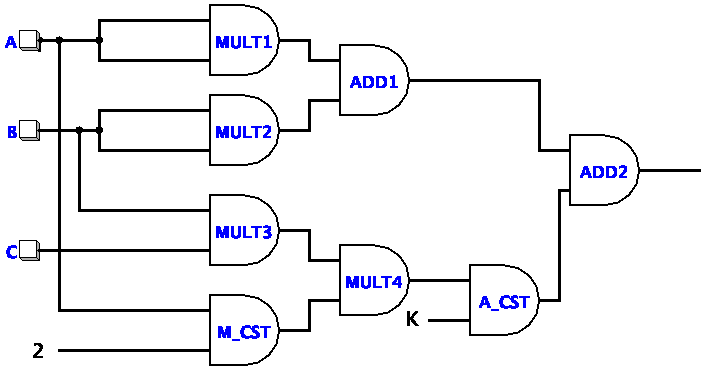
\includegraphics[scale=0.3]{main.png}
\end{itemize}
To run tests for this part, make sure that \textit{trusted} in \textit{mpc\_test.go:25} is set to true.

\section{Part II}
\subsection{Threat model}
The asset to protect for a party is the input. During the protocl, anyone monitoring the communication should not be able to recover the input of a given party. In particular, a party taking part in the computation can not infer more information about another party's input that what he could have infered if all data had been sent to a trusted third-party making the computation for them and sending the result.

All parties follow the "honest but curious" threat model. They do not deviate from the protocol and compute the correct circuit, but try to infer informations about other's input.

In this part, no trusted third-party exist. The parties generates the beaver triplets using homomorphic encryption.
\subsection{Implementation details}
The implementation of this part is identical to the previous part, with the addition of the \textit{beaver.go} file which is used to augment the protocol as follows. : 
\begin{itemize}
    \item Each MPCProtocol now contains a BeaverProtocol which is run before the computation of the circuit, if beaver triplets are needed.
    \item BeaverProtocols communicates using BeaverMessage sent using the same port as MPCMessage. To avoid confusion, BeaverMessage are sent preceded by a $0$ value, while MPCMessage are sent preceded by a $1$ value.
    \item The protocol is then run and works according to the handout specifications.
\end{itemize}

To run tests for this part, make sure that \textit{trusted} in \textit{mpc\_test.go:25} is set to false.
\section{Evaluation}
- Give a comprehensive comparison and evaluation about Part1 and Part2 of the project including performance results. Feel free to use charts, tables, plots...
\begin{itemize}
    \item The addition, addition with a constant, subtraction and multiplication by a constant are gates which compute their respective output locally. A quick glance at the code is necessary to see that they take constant time. The reveal operation as welle as the multiplication (which uses the reveal operation) have to use the network to compute their ouput. Hence they are inherently slower and are directly linked the performance of the circuits.
    %What affects the efficiency of the executions? Be specific, which types of operations/circuits are directly linked to performance?
    \item The difference between Part1 and Part2 is the beaver triplet generation. Part 1 generate them in one place, before the main protocol, acting like a trusted third-party. In Part 2, every party collaborate to generate the triplets. This leads to Part 1 being very efficient whereas Part 2 is order of magnitude slower, since beaver triplets generation requires homomorphic encryption and a lot of network traffic. %Is there any difference in terms of performance between Part I and Part II? Why? 
\end{itemize}

\section{Discussion}
\begin{itemize}
    \item Comment on your findings, discuss different outcomes for each part.
    \item Discuss outcomes from different circuits including your own circuit.
    \item In your opinion, which model is appropriate to use under which conditions/threat model? Why? Discuss.
    \item Come up with a scenario for each part of the implementation, discuss why it makes sense to use homomorphic encryption based generation of Beaver triplets.
\end{itemize}

\section{Conclusion}
\begin{itemize}
    \item Assess your learning outcomes for this project.
    \item What did you do? What did you learn? Any interesting design ideas? 
\end{itemize}

\bibliographystyle{IEEEtran}
\bibliography{bib}
\end{document}
